\documentclass[conference]{IEEEtran}
\IEEEoverridecommandlockouts
% The preceding line is only needed to identify funding in the first footnote. If that is unneeded, please comment it out.
\usepackage{cite}
\usepackage{amsmath,amssymb,amsfonts}
\usepackage{algorithmic}
\usepackage{graphicx}
\usepackage{textcomp}
\usepackage{xcolor}
\def\BibTeX{{\rm B\kern-.05em{\sc i\kern-.025em b}\kern-.08em
    T\kern-.1667em\lower.7ex\hbox{E}\kern-.125emX}}
\begin{document}

\title{Conference Paper Title*\\
{\footnotesize \textsuperscript{*}Note: Sub-titles are not captured in Xplore and
should not be used}
\thanks{Identify applicable funding agency here. If none, delete this.}
}

\author{\IEEEauthorblockN{1\textsuperscript{st} Katrin Glöwing}
\IEEEauthorblockA{\textit{Interaktionstechnik und Design} \\
\textit{Hochschule Hamm-Lippstadt}\\
Lippstadt, Deutschland \\
Immatrikulationsnummer: 2170348}
\and
\IEEEauthorblockN{2\textsuperscript{nd} Domenic Drechsel}
\IEEEauthorblockA{\textit{Interaktionstechnik und Design} \\
\textit{Hochschule Hamm-Lippstadt}\\
Lippstadt, Deutschland \\
Immatrikulationsnummer:2170168}
\and
\IEEEauthorblockN{3\textsuperscript{rd} Justin Frommberger}
\IEEEauthorblockA{\textit{Interaktionstechnik und Design} \\
\textit{Hochschule Hamm-Lippstadt}\\
Lippstadt, Deutschland \\
Immatrikulationsnummer:}
\and
\IEEEauthorblockN{4\textsuperscript{th} Wilms}
\IEEEauthorblockA{\textit{Interaktionstechnik und Design} \\
\textit{Hochschule Hamm-Lippstadt}\\
Lippstadt, Deutschland \\
Immatrikulationsnummer: 2150884}
}

\maketitle

\begin{abstract}
Overview of document including main outcomes
\end{abstract}


\section{Motivation}
%Motivation for project including problem domain and requirements


\section{Sketch of approach}


\section{Concept part}
%From system level specification down to discipline specific
%documentation including diagrams and visualizations \\
%including a comprehensible derivation of your design decisions

\subsection{Szenario}
Der Rescue Roboter wird eingesetzt um Menschen beziehungsweise Lebewesen und Objekte im Fall von Naturkatastrophen oder schweren Unfällen zu retten.
\begin{figure}[htbp] 
  \centering
     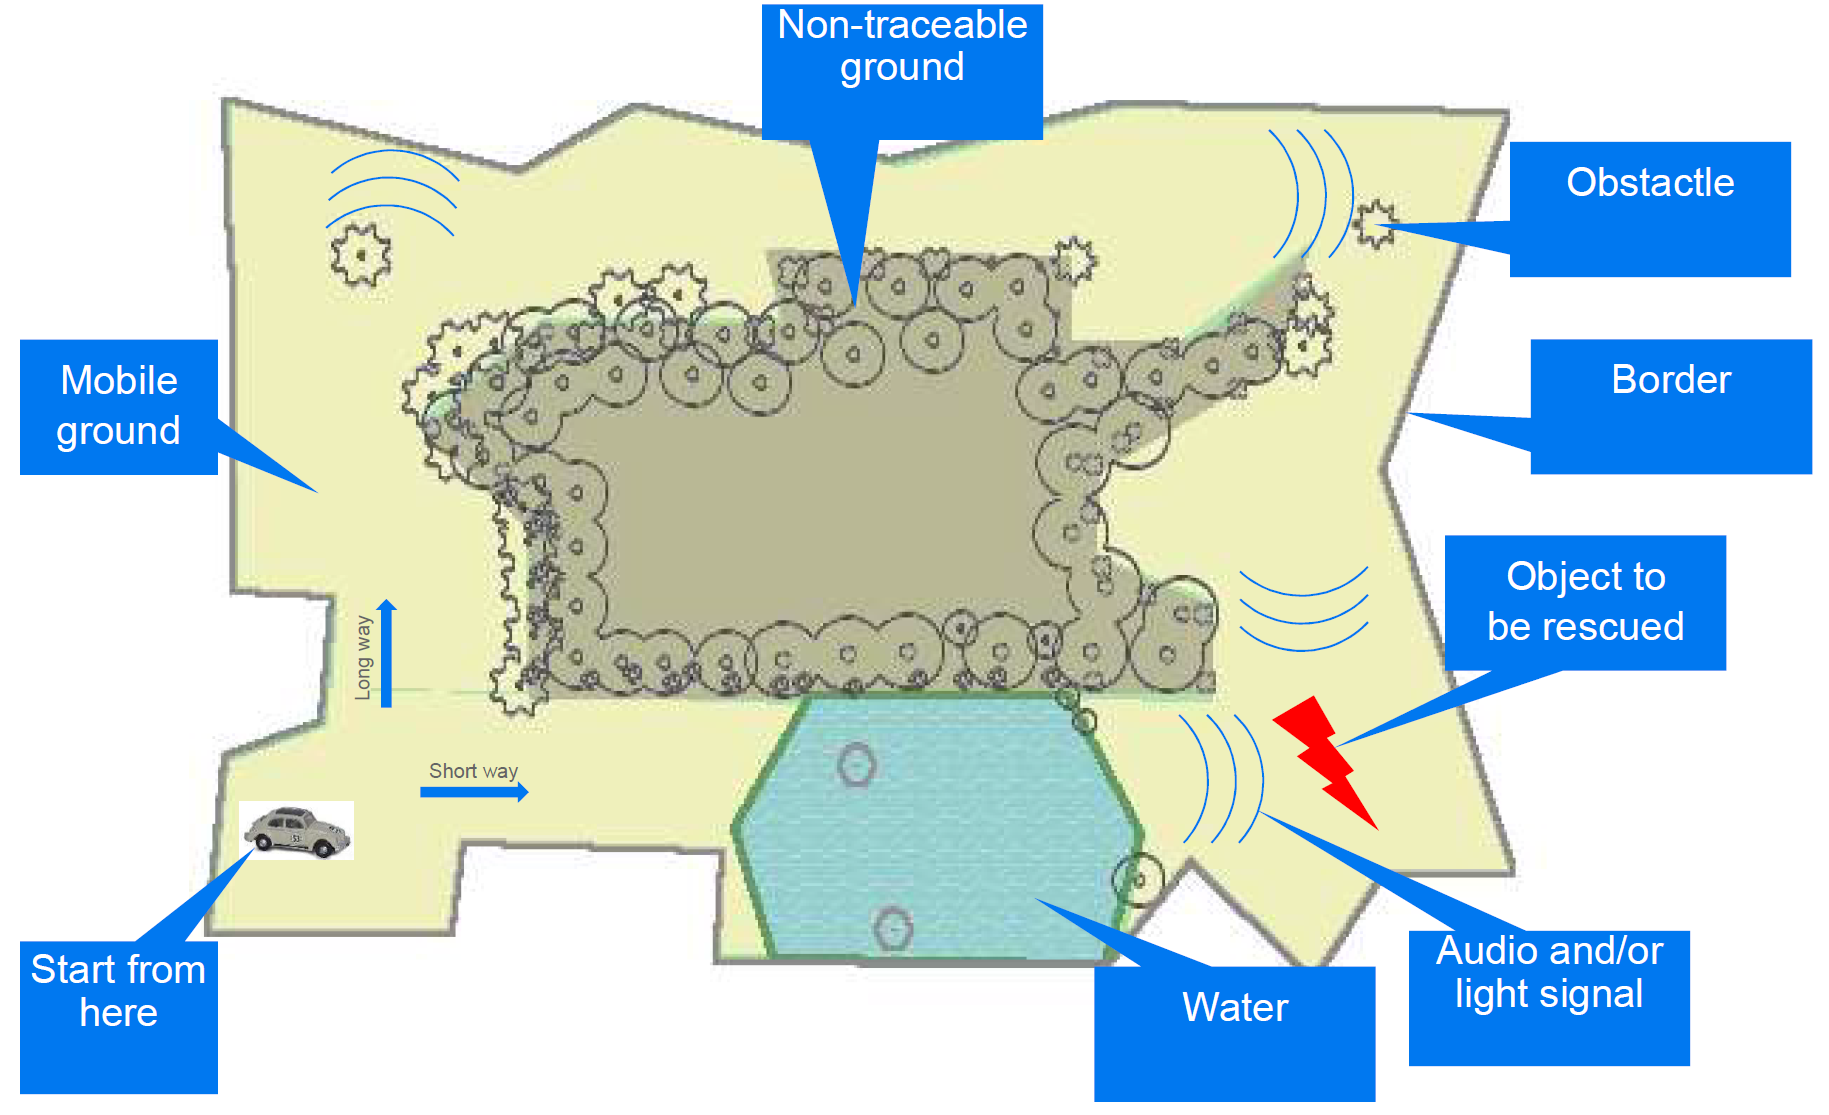
\includegraphics[width=0.5\textwidth]{Bilder/testumgebung.PNG}
  \caption{Testumgebung}
  \label{fig:testumgebung}
\end{figure}\\
Auf der Figur \ref{fig:testumgebung} ist die Testumgebung zu sehen. In diesem Projekt hat der Rescue Roboter die Aufgabe jemanden nach einer Explosion im Mehrfamilienhaus (Figur \ref{fig:testumgebung} "Non-traceable ground") zu bergen. Außerhalb des Hauses finden sich brennende Gegenstände (Figur \ref{fig:testumgebung} "Obstractle") von dem Haus.

\subsection{Anforderungen}
Figur \ref{fig:anforderungen} zeigt die Anforderungen des Projektes.
\begin{figure}[htbp] 
  \centering
     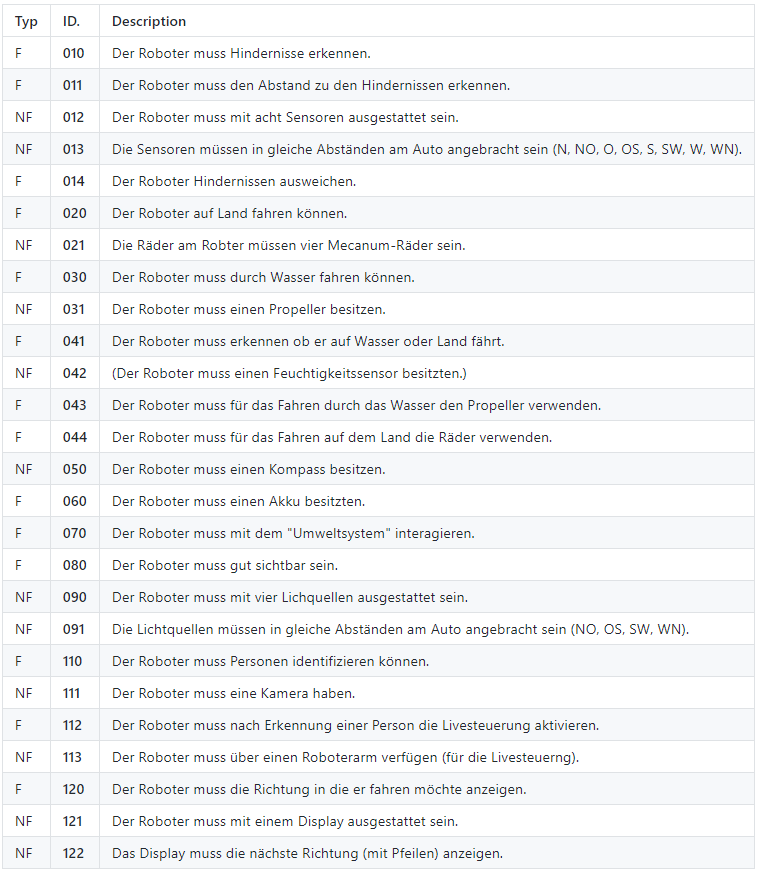
\includegraphics[width=0.5\textwidth]{Bilder/requirements.PNG}
  \caption{Anforderungen}
  \label{fig:anforderungen}
\end{figure}\\
Funktionale Anforderungen (Typ: F) sind Anforderungen die beschreiben was das System oder das Produkt ausführen muss \cite{b1} und nicht-funktionale Anforderungen (Typ: NF) beschreiben die fundamentale Basis der Systemarchitektur \cite{b2}.\\
Das Projekt ist die Simulation eines Rescue Robots.\\
Zusammengefasst sind die Anforderungen folgende: 
\begin{itemize}
    \item Der Roboter muss Hindernisse erkennen und ausweichen.
    \item Der Roboter muss auf Land und Wasser fahren können.
    \item Der Roboter muss seinen Standort weitergeben.
    \item Der Roboter muss anzeigen in welche Richtung er als nächstes fährt.
    \item Der Roboter muss Personen identifizieren.
    \item Der Roboter muss einen Roboterarm besitzen, der per Liveschaltung verwendet wird um Lebewesen und Objekte zu bergen.
\end{itemize}


\section{Evaluation}
%(partly) implementation of system or\\
%partly) Simulation of system e.g. in Matlab or microcontroller-based
%simulation of specific parts, or…


\section{Summary and outlook}

\section{Appendix}

\section{Affidavit}
 % ist vollständig 27.07.2020 KG

\begin{thebibliography}{00}
\bibitem{b1} S. Robertson, and J. Robertson, ``Mastering the Requirements Process: Getting Requirements Right,'' Pearson Education, 2012.
\bibitem{b2} L. Chen and M. Ali Babar and B. Nuseibeh, ``Characterizing Architecturally Significant Requirements,'' IEEE Software, 2nd ed., vol. 30, pp. 38--45, 2013.
\end{thebibliography}
\vspace{12pt}
\color{red}
IEEE conference templates contain guidance text for composing and formatting conference papers. Please ensure that all template text is removed from your conference paper prior to submission to the conference. Failure to remove the template text from your paper may result in your paper not being published.

\end{document}
